As though it was always destined to happen, your team has encountered
the time-traveling eccentric known only as Professor Whatsit. Well, not
so much ``encountered'' as ``collided'', as witnessed by the 
telephone-booth-shaped breach in your starboard hull.

This whacky master of time with a penchant for fezzes and bow ties promises to
repair your ship, but he first needs your help preventing a
Time Crash. You've never heard of this phenomenon before (he describes it as a
``timey-wimey, wibbly-wobbly sort of thing''), but as it seems to be 
related to a puzzle, you agree to pitch in.

Six parallel dimensions are represented by six groups of numbers on
the \textbf{Dimensional Signals} sheet. In every dimension, this solar system
has six planets; the numbers represent how close their orbit reaches their sun.
As it happens, today all six planets will reach that closest
point, forming a straight line. But because this will happen
in all six dimensions simultaneously, all the planets will begin
to warp and eventually merge into each other!
%
%Your task is to associate each group of numbers with a corresponding
%dimensional signal. This signal is constructed by comparing the relative distances
%between adjacent planets when aligned. The six planets begin mutually
%disconnected, but the Time Crash will cause them to warp and overlap,
%eventually merging all the planets into one! 

Thankfully, you can prevent all of this if you can help the Professor
calculate the dimensional signal that would be caused by this dimensional
warp, spelling out a six-letter hidden codeword!
The signal for each dimension represents how
the planets in a dimension would merge as the warping factor increases,
with merged planets represented by bars and isolated planets represented
by dots (with order not mattering). 
The illustration below demonstrates this effect for \texttt{06-24-32-55-70-99},
matching the signal labeled \texttt{E}.

\begin{center}
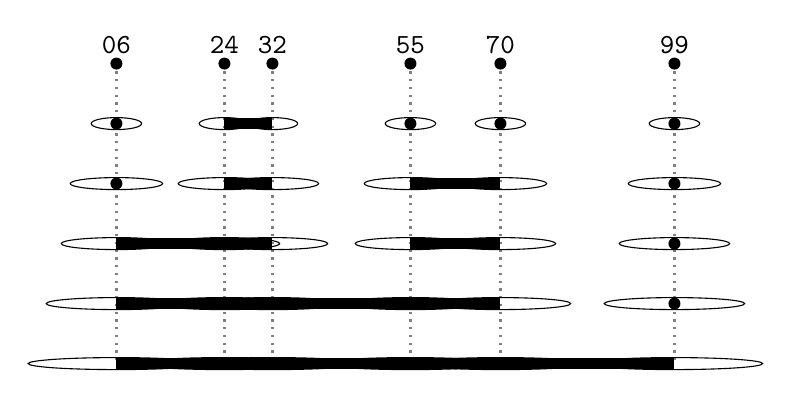
\begin{tikzpicture}[x=0.3in,y=0.3in] 
%\node[left] at (-1,0) {No Warp Factor};
%\node[left] at (-1,-1) {Warp Factor \(4\)};
%\node[left] at (-1,-2) {Warp Factor \(7.5\)};
%\node[left] at (-1,-3) {Warp Factor \(9\)};
%\node[left] at (-1,-4) {Warp Factor \(11.5\)};
%\node[left] at (-1,-5) {Warp Factor \(14.5\)};
\draw[thick,black!50,dotted] (0.6,0) -- +(0,-5);
\draw[thick,black!50,dotted] (2.4,0) -- +(0,-5);
\draw[thick,black!50,dotted] (3.2,0) -- +(0,-5);
\draw[thick,black!50,dotted] (5.5,0) -- +(0,-5);
\draw[thick,black!50,dotted] (7.0,0) -- +(0,-5);
\draw[thick,black!50,dotted] (9.9,0) -- +(0,-5);
\fill (0.6,0) circle (0.1) node[above] {\texttt{06}};
\fill (2.4,0) circle (0.1) node[above] {\texttt{24}};
\fill (3.2,0) circle (0.1) node[above] {\texttt{32}};
\fill (5.5,0) circle (0.1) node[above] {\texttt{55}};
\fill (7.0,0) circle (0.1) node[above] {\texttt{70}};
\fill (9.9,0) circle (0.1) node[above] {\texttt{99}};
\begin{scope}[shift={(0,-1)}]
\draw (0.6,0) ellipse (0.42 and 0.1); 
\draw (2.4,0) ellipse (0.42 and 0.1); 
\draw (3.2,0) ellipse (0.42 and 0.1); 
\draw (5.5,0) ellipse (0.42 and 0.1); 
\draw (7.0,0) ellipse (0.42 and 0.1); 
\draw (9.9,0) ellipse (0.42 and 0.1); 
\fill (0.6,0) circle (0.1); 
\draw[line width=4pt] (2.4,0) -- (3.2,0);
\fill (5.5,0) circle (0.1);
\fill (7.0,0) circle (0.1);
\fill (9.9,0) circle (0.1);
\end{scope}
\begin{scope}[shift={(0,-2)}]
\draw (0.6,0) ellipse (0.77 and 0.1); 
\draw (2.4,0) ellipse (0.77 and 0.1); 
\draw (3.2,0) ellipse (0.77 and 0.1); 
\draw (5.5,0) ellipse (0.77 and 0.1); 
\draw (7.0,0) ellipse (0.77 and 0.1); 
\draw (9.9,0) ellipse (0.77 and 0.1); 
\fill (0.6,0) circle (0.1); 
\draw[line width=4pt] (2.4,0) -- (3.2,0);
\draw[line width=4pt] (5.5,0) -- (7.0,0);
\fill (9.9,0) circle (0.1);
\end{scope}
\begin{scope}[shift={(0,-3)}]
\draw (0.6,0) ellipse (0.92 and 0.1); 
\draw (2.4,0) ellipse (0.92 and 0.1); 
\draw (3.2,0) ellipse (0.92 and 0.1); 
\draw (5.5,0) ellipse (0.92 and 0.1); 
\draw (7.0,0) ellipse (0.92 and 0.1); 
\draw (9.9,0) ellipse (0.92 and 0.1); 
\draw[line width=4pt] (0.6,0) -- (3.2,0);
\draw[line width=4pt] (5.5,0) -- (7.0,0);
\fill (9.9,0) circle (0.1);
\end{scope}
\begin{scope}[shift={(0,-4)}]
\draw (0.6,0) ellipse (1.17 and 0.1); 
\draw (2.4,0) ellipse (1.17 and 0.1); 
\draw (3.2,0) ellipse (1.17 and 0.1); 
\draw (5.5,0) ellipse (1.17 and 0.1); 
\draw (7.0,0) ellipse (1.17 and 0.1); 
\draw (9.9,0) ellipse (1.17 and 0.1); 
\draw[line width=4pt] (0.6,0) -- (7.0,0);
\fill (9.9,0) circle (0.1);
\end{scope}
\begin{scope}[shift={(0,-5)}]
\draw (0.6,0) ellipse (1.47 and 0.1); 
\draw (2.4,0) ellipse (1.47 and 0.1); 
\draw (3.2,0) ellipse (1.47 and 0.1); 
\draw (5.5,0) ellipse (1.47 and 0.1); 
\draw (7.0,0) ellipse (1.47 and 0.1); 
\draw (9.9,0) ellipse (1.47 and 0.1); 
\draw[line width=4pt] (0.6,0) -- (9.9,0);
\end{scope}
\end{tikzpicture}
\end{center} 
